The previous chapter introduced motion planning problems that are formulated with respect to the robot's configuration space ($C$-space). In particular, two specific approaches for motion planning in $C$-space were discussed: grid-based methods and combinatorial planning methods. Grid-based methods discretize the continuous $C$-space into a grid, and then use graph search methods such as A* to compute paths through the grid. Combinatorial planners compute a \textit{roadmap} that consists of a finite set of points in the $C$-space, but avoids the use of a rigid grid structure. Planning with the roadmap then consists of connecting the initial configuration and desired configuration to the roadmap, and then performing a graph search to find a path along the roadmap.

Generally speaking, grid-based methods suffer from the rigidity of the discretization that is performed. In contrast, combinatorial planners have much more flexibility because \textit{any} configuration $q$ can be a part of the roadmap. However, both types of planners require a complete characterization of the free configuration space (e.g. points in the configuration space that don't result in a collision with obstacles) in advance. In this chapter, a class of motion planning algorithms is presented which builds a roadmap that is similar to combinatorial planners, but without requiring a full characterization of the free configuration space. Instead, these algorithms build roadmaps one point at a time by sampling a point in the configuration space, and then querying an independent module to determine if the sample is admissible. This class of planners are referred to as \textit{sampling-based methods}\cite{LaValle2006}.


\notessection{Sampling-Based Motion Planning}
In contrast to the search-based motion planners discussed in the last chapter, sampling-based methods leverage an independent module that can be queried to determine if a configuration is admissible. In the context of robotics, an admissible configuration in motion planning problems is often one that is collision-free and therefore this module is often referred to as a collision detection module (or simply a \textit{collision checker}).
The collision detection module is used to probe and incrementally build a roadmap in the configuration space, rather than attempting to completely characterize the free space in advance (as is done in combinatorial planners). 

Sampling-based algorithms are a common choice for practical applications as they are conceptually simple, flexible, relatively easy to implement, and can be extended beyond the geometric case (i.e. they can consider differential constraints). The disadvantages of the approach are typically with respect to theoretical guarantees, for example these approaches cannot certify that a solution doesn't exist. In this chapter the focus will be on two popular sampling-based methods: probabilistic roadmaps (PRM) and the rapidly-exploring random trees (RRT) algorithm. Additional techniques such as the fast-marching tree algorithm (FMT*), kinodynamic planning, and deterministic sampling-based methods will also be briefly mentioned. 

\subsection{Probabilistic Roadmap (PRM)}
It is easiest to start with the probabilistic roadmap algorithm because it is conceptually quite similar to combinatorial planners from the previous section. In particular, the PRM algorithm also generates a topological graph $G$ called a \textit{roadmap} where the vertices are configurations $q$ in the free part of the configuration space $C_{free}$, and edges connect the vertices (and must also entirely lie in $C_{free}$). Once the roadmap is generated, a motion plan can be found for a given initial configuration $q_I$ and goal configuration $q_G$ by first connecting them to the roadmap, and then using a graph-search algorithm (e.g. A*) to find a path along the roadmap graph $G$. The difference between PRM and combinatorial planners lies in the method in which the roadmap is generated.

The key insight of the PRM algorithm is that a complete characterization of the free configuration space (which is computationally expensive) can be avoided by sampling configurations $q$ at random and then using a collision checker to validate if $q \in C_{free}$. The general outline of the algorithm follows:
\begin{enumerate}
    \item Randomly sample $n$ configurations $q_i$ from the configuration space.
    \item Query a collision checker for each $q_i$ to determine if $q_i \in C_{free}$, if $q_i \not\in C_{free}$ then it is removed from the sample set.
    \item Create a graph $G = (V,E)$ with vertices from the sampled configurations $q_i \in C_{free}$. Define a radius $r$ and create edges for every pair of vertices $q$ and $q'$ where: (i) $\lVert q - q' \rVert \leq r$ and (ii) the straight line path between $q$ and $q'$ is also collision free.
\end{enumerate}
An example of the roadmap resulting from applying this algorithm is shown in Figure \ref{fig:prm-graph}.
\begin{figure}[ht]
  \centering
   \includegraphics[width=0.65\textwidth]{tex/figs/ch06_figs/prm.png}
  \caption{Example solution found via the PRM algorithm. The black dots represent the randomly sampled vertices of the graph, and the grey lines represent the edges created between vertices within a predefined radius $r$ of each other. The initial configuration $q_{start}$ and goal configuration $q_{goal}$, are connected through this roadmap along the pink line, which is found by a graph-search algorithm.}
  \label{fig:prm-graph}
\end{figure}
Note that using the \textit{connectivity radius} $r$ is a simple and efficient way of connecting the sampled vertices without having a burdensome number of edges. This is desirable because having too many edges is unnecessary, will make the graph-search more challenging, and will require more collision checks to be made\footnote{Edge validation is usually performed by densely sampling the edge and checking for collisions at each.}. On the flip side, making the radius $r$ too small could mean not enough connections are made.

The downside of PRM is that finding good solutions may require a large number of samples $n$ to sufficiently cover the configuration space. Similar to why having too many edges is not good, having too many samples will require a lot of queries of the collision checker, which may be costly. However, there are some scenarios where building a roadmap that completely covers the space $C_{free}$ is beneficial, namely in \textit{multi-query} planning problems. In multi-query problems, it is assumed that the motion planner will be called many times for different initial $q_I$ and goal $q_G$ configurations. In this case the PRM graph can be built once to cover $C_{free}$, and then it can be reused as many times as needed. In other words, the costly sampling and collision checking only needs to be done once at the start, so it may be worth the ``investment''. Note however that this only works if the environment stays the same in between each query of the motion planner. If the environment changes, the entire PRM roadmap would have to be rebuilt from scratch!

\subsection{Rapidly-exploring Random Trees (RRT)}
In multi-query problems where the environment does not change in between each query, the probabilistic roadmap (PRM) algorithm offers the advantage of front-loading some work to provide efficient queries later. However, many problems in robotics are alternatively classified as \textit{single-query} problems, where it is assumed that only a single query will be made to the motion planner. A common single-query planning scenario arises from changing environments, such as if there is a moving obstacle. In this case building up a roadmap over the entire free configuration space $C_{free}$ may result in wasted effort. The RRT algorithm solves this problem by incrementally sampling and building the graph, starting at the initial configuration $q_I$, until the goal configuration $q_G$ is reached. Additionally, the graph is built as a \textit{tree}, which is a special type of graph that has only one path between any two vertices in the graph.

In general, the RRT algorithm begins by initializing a tree\footnote{The tree is a graph, however since it has special structure it is denoted as $T$ rather than $G$.} $T = (V,E)$ with a vertex at the initial configuration (i.e. $V = \{q_I\}$). At each iteration the RRT algorithm then performs the following steps:
\begin{enumerate}
    \item Randomly sample a configuration $q \in C$.
    \item Find the vertex $q_{near} \in V$ that is closest to the sampled configuration $q$.
    \item Compute a new configuration $q_{new}$ that lies on the line connecting $q_{near}$ and $q$ such that the entire line from $q_{near}$ to $q_{new}$ is contained in the free configuration space $C_{free}$.
    \item Add a vertex $q_{new}$ and an edge $(q_{near}, q_{new})$  to the tree $T$.
\end{enumerate}
Thus after each iteration only a single point is sampled and potentially added to the tree. Additionally, every so often the sampled point $q$ can be set to be the goal configuration $q_G$. Then, if the nearest point $q_{near}$ can be connected to $q_G$ by a collision-free line the search can be terminated. Intuitively, this approach works because of a phenomenon referred to as the \textit{Voronoi bias}, which essentially describes the fact that there is more ``empty space'' near the nodes on the frontier of the tree. Therefore, a randomly sampled point is more likely to be drawn in this ``empty space'', causing the frontier to be extended (and therefore driving exploration).

Note that variations on this standard algorithm exist, in particular there exist different ways of connecting a sampled point to the existing tree. One popular variant that modifies the way a sampled point is connected to the tree is known as RRT* (pronounced RRT star). This modified RRT algorithm introduces a notion of optimality into the planner and will in fact return an optimal solution as the number of samples approaches infinity. Another variant of RRT is called RRT-Connect, which simultaneously builds a tree from both the initial configuration $q_I$ and the goal configuration $q_G$ and tries to connect them.

\begin{figure}[ht]
  \centering
  
\includegraphics[width=0.65\textwidth]{tex/figs/ch06_figs/rrt.png}
  \caption{Example exploration tree by the RRT algorithm. The black dots represent points sampled at each iteration of the algorithm, which are connected to the nearest vertex that is currently part of the tree.}
  \label{fig:rrt-graph}
\end{figure}

\subsection{Theoretical Results for PRM and RRT}
One of the main challenges of sampling-based motion planning is that it is unclear how many samples are needed to find a solution. However, some theoretical guarantees can be provided regarding their asymptotic behavior (i.e. behavior as number of samples $n \xrightarrow{} \infty$). In particular, both PRM\footnote[][-8\baselineskip]{With a constant connectivity radius $r$.} and RRT are guaranteed\footnote[][-8\baselineskip]{These guarantees also require an assumption that the configuration space is bounded, for example if $C$ is the $d$-dimensional unit hypercube with $2 \leq d \leq \infty$.} to eventually find a solution if it exists \cite[-4\baselineskip]{LaValle1998}\cite[-\baselineskip]{KavrakiSvestkaEtAl1996}.
Regarding solution \textit{quality}, it has been shown that PRM (with the appropriate choice of the radius $r$) can find optimal paths as the number of samples $n \xrightarrow{} \infty$. However, RRT can be arbitrarily bad with non-negligible probability \cite{KaramanFrazzoli2011}.

\subsection{Fast Marching Tree Algorithm (FMT*)}
As previously mentioned, PRM is an asymptotically optimal algorithm which means that with enough samples it will find good paths. However, in practice PRM with a large number of samples also requires a lot of collision checks and is therefore costly. On the other hand, RRT is fast but in general will not find good paths.
FMT* is a an advanced sampling-based motion planning algorithm that maintains the advantages of both of these algorithms (i.e. fast and asymptotically optimal) \cite{JansonSchmerlingEtAl2015}.

FMT* builds a tree structured graph in the same way RRT does (which maintains the efficiency of RRT), but makes connections in a way that allows for asymptotic optimality. In particular, the technique used for making new connections is referred to as \textit{dynamic programming}. Dynamic programming can be used to find the best paths with respect to a \textit{cost-of-arrival}, denoted $c(q)$, which represents the cost to move from the initial configuration $q_I$ to the configuration $q$. An example of a common metric is simply the Euclidean distance, which would result in a ``shortest'' path. In the context of motion planning, dynamic programming leverages Bellman's \textit{principle of optimality}, which states that the optimal paths satisfy:
\begin{equation}
\label{eq:bellmancost}
c(v) = \min_{u:\lVert u - v\rVert < r_n} \text{Cost}(u, v) + c(u),
\end{equation}
where $u$ are nodes within radius $r_n$ of node $v$, $\text{Cost}(u, v)$ is the cost of an edge between $u$ and $v$, and $c(u)$ is the cost-to-arrive at $u$. In words, this relationship says that the cost-of-arrival at any configuration $v$ on the optimal path is defined by searching over all local neighboring configurations to find which would result in the best path. FMT* uses this principle repeatedly every time it needs to connect a new sample to the tree.
However, in practice using the condition \eqref{eq:bellmancost} is complicated by the fact that the resulting edge may result in a collision. FMT* handles this by ignoring obstacles when using the condition \eqref{eq:bellmancost} to connect a new sample to the tree, and then if a collision occurs from the resulting connection it is simply skipped and the algorithm moves on to a new sample. Therefore this application of dynamic programming is referred to as \textit{lazy} because it only checks for collisions after the fact. It turns out that this substantially reduces the total amount of collision checks required, and only leads to sub-optimality in rare cases.


\begin{figure}[ht]
  \centering
  \includegraphics[width=0.75\textwidth]{tex/figs/ch06_figs/fmt.png}
  \caption{Example of a step in FMT*. Suppose the sample $v$ has been selected to be the next point to be added to the tree. The candidate costs $\text{Cost}(u_1, v) + c(u_1)$ and $\text{Cost}(u_2, v) + c(u_2)$ are evaluated to see which connection would minimize $c_v$. Suppose $u_2$ was selected by this criteria (i.e. $u_2$ satisfies \eqref{eq:bellmancost}), then the collision checker would see that the edge $(u_2,v)$ results in a collision and the sample $v$ would be skipped (but could be added later).}
  \label{fig:plot_idea}
\end{figure}

\subsection{Kinodynamic Planning}
The geometric motion planning algorithms previously considered assume that the robot does not have any constraints on its motion and only a collision-free solution is required. This makes the planning task easier because two configurations $q$ and $q'$ can be simply connected by the planner with a \textit{straight line}. However, robots do typically have kinematic/dynamical constraints on their motion, and for some motion planning problems it is desirable or even necessary to take those constraints into account.
The problem of planning a path through the free configuration space $C_{free}$ that satisfies a given set of differential constraints is referred to as \textit{kinodynamic motion planning}\cite{SchmerlingJansonEtAl2015}. 

Similar to previous chapter, it is assumed that the robot operates in a state space $X\subseteq R^n$ and can apply controls $\bu \in U \subseteq \R^m$, and that the motion constraints are given by the differential model (i.e. from kinematic or dynamics constraints):
\begin{equation} \label{eq:dmodel}
\dot{\x} = f(\x,\bu),
\end{equation}
where $\x \in \R^n$ and $\bu \in \R^m$. Note that the state space $X$ is not necessarily the same as the configuration space $C$, but the configuration $q$ is derivable from the state $x$. As was previously mentioned, the configuration space is something that can be chosen to capture the information that is necessary for obstacle avoidance. However to include dynamics constraints it is required that the motion planning now be done in the state space $X$.

The RRT algorithm can be extended to the kinodynamic case with relative simplicity. In particular, a random state $x$ is sampled from the state space $X$ and its nearest neighbor $x_{near}$ on the current tree $T$ is found. Instead of connecting $x$ and $x_{near}$ with a straight line (which is likely not dynamically feasible), a random control $u \in U$ and random time $t$ are sampled. Then, the state is propagated forward by integrating the differential equations \eqref{eq:dmodel} with the chosen $u$ for a time $t$ and initial condition $x_{near}$. The resulting state $x_{new}$ is then added to the tree if the path from $x_{near}$ to $x_{new}$ is collision free. This is referred to as a \textit{forward-propagation-based} approach.

Another approach to kinodynamic planning leverage \textit{steering-based} algorithms. In these approaches, the planner selects two points in the state space $x$ and $x'$ and then uses a steering subroutine to find a feasible trajectory to connect these points. Crucially, these approaches only work well if the steering subroutine is \textit{efficient}. This approach is be particularly well suited for differential flat systems.

\begin{figure}[ht]
    \centering
    \begin{subfigure}[b]{0.4\linewidth}
      \includegraphics[width=\linewidth]{tex/figs/ch06_figs/driftless.png}
      \caption{Reeds-Shepp car}
    \end{subfigure}
    \begin{subfigure}[b]{0.4\linewidth}
      \includegraphics[width=\linewidth]{tex/figs/ch06_figs/drift.png}
      \caption{Double integrator system}
    \end{subfigure}
    \caption{Results from a kinodynamic planner called Differential FMT* (DFMT*) (Schmerling et al.). The figure on the left shows the results for a Reeds-Shepp car model, and on the right is a double integrator model.}
    \label{fig:kino}
\end{figure}


\subsection{Deterministic Sampling-Based Motion Planning}

Probabilistic sampling-based algorithms, such as the probabilistic roadmap (PRM) and the rapidly exploring random tree (RRT) algorithms, have been quite successful in practice for robotic motion planning and often have nice theoretical properties (e.g. in terms of probabilistic completeness or even asymptotic optimality). Such algorithms are \textit{probabilistic} because they compute a path by connecting independently and identically distributed (i.i.d.) random points in the configuration space. However, this randomization introduces several challenges for practical use, including certification for safety-critical applications and the ability to use offline computation to improve real-time execution. Hence, it is important to ask whether similar (or better) theoretical guarantees and practical performance could be obtained by considering \textit{deterministic} approaches.

An important metric for answering this question is referred to as the $l_2$-dispersion. 
\begin{definition}[$l_2$-dispersion]
For a finite set $S$ of points contained in $X \subset R^d$, its $l_2$-dispersion $D(S)$ is defined as:
\begin{equation}
    D(S) := \underset{x\in X}{\text{sup}}\: \underset{ s \in S}{\text{min}} \lVert s - x \rVert_2.
\end{equation}
\end{definition}
Intuitively, the $l_2$-dispersion of $S$ quantifies how well a space is covered by the set of points in $S$ in terms of the largest Euclidean ball that touches and contains none of the points. For a fixed number of samples, a small $l_2$-dispersion (only a small radius ball can be fit among the points of $S$ without touching or containing any) means that the points are more uniformly distributed. 

To create a deterministic sampling based motion planning algorithm, it is desirable to generate a set of samples $S$ with low-dispersion. In fact, low-dispersion sampling sequences exist that give sets $S$ with $l_2$-dispersion $D(S)$ on the order of $O(n^{-1/d})$ where $d$ is the dimension of the space. Additionally, for $d=2$ it is possible to create sequences of points $S$ that \textit{minimize} the $l_2$-dispersion. Then, if the set $S$ of $n$ samples has $l_2$-dispersion that satisfies
\begin{equation*}
    D(S) \leq \gamma n^{-1/d},
\end{equation*}
for some $\gamma > 0$, and if $\lim_{n\rightarrow\infty}n^{1/d}r_n = \infty$, then the arc length of the path $c_n$ returned will converge to the optimal path $c^*$ as $n \xrightarrow{} \infty$.

In summary, deterministic sampling can be used to generate motion planning algorithms. These deterministic algorithms still maintain the asymptotic optimality guarantees that probabilistic planners do, and can even use a smaller connection radius $r_n$.


\subsection{Exercises}
All exercises for this chapter can be found in the online repository:

\vspace{\baselineskip}

\url{https://github.com/PrinciplesofRobotAutonomy/AA274A_HW2}.

\subsubsection{Rapidly-Exploring Random Trees}
Complete \textit{Problem 2: Rapidly-Exploring Random Trees (RRT)}, where you will implement the RRT sample-based motion planning algorithm to plan paths in simple 2D environments. Additionally, in this problem you will start with a simple geometric planner that does not consider robot dynamics, but will then extend the RRT algorithm to consider a wheeled robot modeled with Dubins car dynamics. 

\subsubsection{Motion Planning \& Control}
Complete \textit{Problem 3: Motion Planning \& Control}, where you will combine an A* planner with a differential flatness-based tracking controller and a pose stabilization controller to enable a unicycle robot to autonomously move through a 2D environment. Note that this problem requires exercises from previous chapters to be completed first.

\subsubsection{Bi-Directional Sampling-based Motion Planning}
Complete \textit{Extra Problem: Bi-Directional Sampling-based Motion Planning}, where you will implement a variation of the RRT algorithm known as RRT-Connect, which uses a bi-direction approach to building the RRT tree. This algorithm will be implemented for both a simple geometric path planner as well as for a Dubins car robot.